\chapter{SMAWK}
\label{SMAWK}

%----------------------------------------------------------------------------------------

Neste capítulo discutiremos o algoritmo SMAWK. Este algoritmo tem a mesma função da otimização divisão e conquista, porém, precisa que a matriz seja totalmente monótona, não apenas monótona, e tem uma complexidade assintótica melhor do que aquele. Ele é conhecido pela sua aplicação no problema de encontrar um vértice mais distante de cada vértice num polígono convexo em tempo linear~\cite{Aggarwal:1987}, mas pode ser usado em vários outros problemas, assim como a otimização da divisão e conquista.

Dada uma matriz $A \in \B{Q}^{n \times m}$, listamos os casos em que este algoritmo se aplica:
\begin{itemize}
    \item Se $A$ é totalmente monótona convexa ou côncava nas linhas, podemos encontrar os índices de mínimos e máximos das linhas em tempo $\Cl{O}(n + m)$;
    \item Se $A$ é totalmente monótona convexa ou côncava nas colunas, podemos encontrar os índices de mínimos e máximos das colunas em tempo $\Cl{O}(n + m)$.
\end{itemize}

Apresentaremos o caso onde $A$ é totalmente monótona convexa nas linhas e estamos interessados nos índices de mínimos. É fácil manipular o algoritmo para trabalhar com os outros casos.

%----------------------------------------------------------------------------------------

\section{Técnica primordial} \label{SMAWK:primordial}
Para facilitar a compreensão do algoritmo SMAWK, iremos apresentar uma técnica parecida com a otimização da divisão e conquista, apresentada no Capítulo~\ref{DivConq}, e mostrar uma otimização desta técnica que leva ao algoritmo SMAWK.

Dada uma matriz~$A \in \B{Q}^{n \times m}$ totalmente monótona convexa por linhas, queremos encontrar o índice de mínimo de cada uma das linhas de~$A$. Se, para uma dada linha~${ i \in [2 \tdots n-1] }$, conhecermos os índices~$\ell$ e~$r$ de mínimos das linhas~${ i-1 }$ e~${ i+1 }$, sabemos, pela monotonicidade de~$A$ que o índice de mínimo da linha~$i$ está em~${ [\ell \tdots r] }$. Além disso, se~${ i = 1 }$ e~${ \ell = 1 }$ ou se~${ i = n }$ e~${ r = m }$, o resultado descrito continua valendo.

Já que~$A$ é totalmente monótona, remover qualquer linha de~$A$ mantém a total monotonicidade e não altera o índice de mínimo de outra linha. Graças a este fato, podemos remover todas as linhas pares da matriz, encontrar os mínimos recursivamente para todas as linhas restantes e depois utilizar as respostas conhecidas para calcular os índices de mínimos das linhas pares. Vamos mostrar que esta última parte, encontrar os mínimos das linhas pares dados os mínimos das outras, custa tempo~$\Cl{O}(n+m)$.

\begin{figure}[h]
    \centering
    % === Based On ===
% Geometric representation of the sum 1/4 + 1/16 + 1/64 + 1/256 + ...
% Author: Jimi Oke
% ================

\begin{tikzpicture}[scale=.35]\footnotesize

\begin{scope}[yscale=-1] % I'm flipping the y-axis because I'm working on grids
  % Step 1
  \pgfmathsetmacro{\p}{0} % initial x

  \foreach \i in {0,...,3} {
    \draw[step=1cm,gray,very thin] (\p,\i+\i) grid (\p+7,\i+\i+1); % grid
  }

  % Step 2
  \pgfmathsetmacro{\p}{10}

  \foreach \i in {0,...,3} {
    \draw[step=1cm,gray,very thin] (\p,\i+\i) grid (\p+7,\i+\i+1);
  }

  \fill[pattern=north west lines,pattern color=red] (\p,0) rectangle (\p+1,1);
  \fill[pattern=north west lines,pattern color=red] (\p+2,2) rectangle (\p+3,3);
  \fill[pattern=north west lines,pattern color=red] (\p+5,4) rectangle (\p+6,5);
  \fill[pattern=north west lines,pattern color=red] (\p+6,6) rectangle (\p+7,7);

  % Step 3
  \pgfmathsetmacro{\p}{20}
  \draw[step=1cm,gray,very thin] (\p,0) grid (\p+7,7);

  \fill[pattern=north west lines,pattern color=red] (\p,0) rectangle (\p+1,1);
  \fill[pattern=north west lines,pattern color=red] (\p+2,1) rectangle (\p+3,2);
  \fill[pattern=north west lines,pattern color=red] (\p+2,2) rectangle (\p+3,3);
  \fill[pattern=north west lines,pattern color=red] (\p+3,3) rectangle (\p+4,4);
  \fill[pattern=north west lines,pattern color=red] (\p+5,4) rectangle (\p+6,5);
  \fill[pattern=north west lines,pattern color=red] (\p+5,5) rectangle (\p+6,6);
  \fill[pattern=north west lines,pattern color=red] (\p+6,6) rectangle (\p+7,7);

  \draw[green,thick] (\p,1) rectangle (\p+3,2);
  \draw[green,thick] (\p+2,3) rectangle (\p+6,4);
  \draw[green,thick] (\p+5,5) rectangle (\p+7,6);
\end{scope}

\end{tikzpicture}

    \caption{Progresso da técnica primordial. Primeiro, as linhas pares são removidas da matriz original. Depois os mínimos das linhas restantes, hachurados em vermelho, são definidos recursivamente. Finalmente, as linhas pares são restauradas e as posições circuladas em verde são percorridas em busca dos seus mínimos, em vermelho.} 
\end{figure}

Definimos, para cada~$i$ ímpar, o valor~$t_i$ que representa o índice de mínimo da~$i$-ésima linha, além dos valores~${ t_0 = 1 }$ e, caso~$n$ seja par, o valor~${ t_{n+1} = m }$. Para cada linha~$i$ par, o parágrafo anterior sugere buscar o mínimo desta linha entre as posições~$t_{i-1}$ e~$t_{i+1}$. Podemos escrever o tempo gasto para encontrar o mínimo de cada uma das linhas pares como~${ \sum\limits_{ i \in [n] \text{ par} }( t_{i+1} - t_{i-1} ) }$ e concluir, desta expressão, que o tempo gasto ao todo é~$\Cl{O}(n+m)$. 

Considerando que remover todas as linhas pares de uma matriz pode ser realizado em tempo~$\Cl{O}(1)$, é fácil ver que o tempo de execução total deste algoritmo é~$\Cl{O}((n+m)\lg(n)$, já que só é possível remover todas as linhas pares~$\Cl{O}(\lg(n))$ vezes.

%----------------------------------------------------------------------------------------

\section{Reduce} \label{SMAWK:reduce}
Chamamos de ótimas as células de uma matriz que são o mínimo de alguma linha e as colunas que contém pelo menos uma célula ótima. Lembre que a definição de mínimo permite apenas um mínimo por linha, portanto, uma matriz contém no máximo~$n$ colunas ótimas.

Queremos agilizar a técnica apresentada acima. Para isso, vamos adicionar a nova hipótese de que a matriz~$A$ é quadrada, ou seja,~$n = m$. A cada passo, removemos as~$\floor{n/2}$ linhas pares da matriz, gerando uma nova matriz $A'$, resolvemos o problema recursivamente em~$A'$ e usamos a solução de~$A'$ para encontrar os mínimos das linhas restantes de~$A$. Quando removemos linhas da nossa~$A$, ela deixa de ser quadrada e passa a ser uma matriz com mais colunas do que linhas, isto é,~$m \geq n$. Queremos remover colunas não ótimas dessa matriz com mais colunas do que linhas fazendo com que a matriz resultante se torne quadrada.  

Vamos desenvolver o algoritmo \textsc{Reduce} a partir de um índice de linha~$k$ e de algumas invariantes: 
\begin{enumerate}
    \item $k \in [1 \tdots n]$, \label{invar:Reduce0}
    \item apenas colunas não ótimas foram removidas da matriz e \label{invar:Reduce1}
    \item toda célula em uma coluna de índice menor ou igual a~$k$ que possua índice de linha menor do que seu índice de coluna não é ótima. \label{invar:Reduce2}
\end{enumerate}

\begin{figure}[h]
    \centering
    % === Based On ===
% Geometric representation of the sum 1/4 + 1/16 + 1/64 + 1/256 + ...
% Author: Jimi Oke
% ================

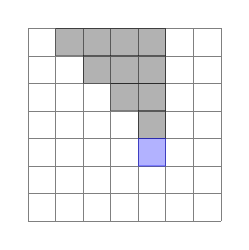
\begin{tikzpicture}[scale=.35]\footnotesize
 \pgfmathsetmacro{\xone}{0}
 \pgfmathsetmacro{\xtwo}{7}
 \pgfmathsetmacro{\yone}{0}
 \pgfmathsetmacro{\ytwo}{7}

\begin{scope}<+->;
% grid
  \draw[step=1cm,gray,very thin] (\xone,\yone) grid (\xtwo,\ytwo);
\end{scope}

% function
\begin{scope}[thin,black,opacity=.3]
  \filldraw (1,7) rectangle (5,6);
  \filldraw (2,6) rectangle (5,5);
  \filldraw (3,5) rectangle (5,4);
  \filldraw (4,4) rectangle (5,3);
  \filldraw[blue] (4,3) rectangle (5,2);
\end{scope}

\end{tikzpicture}

    \caption{Invariante~\ref{invar:Reduce2} do \textsc{Reduce}. A célula~$(k,k)$ está preenchida em azul. As células que, segundo a Invariante~\ref{invar:Reduce2}, não são ótimas estão pontilhadas em preto.} \label{figure:Reduce1}
\end{figure}

Vamos comparar~$A[k][k]$ com~$A[k][k+1]$ e considerar dois casos. Em cada um dos casos, concluiremos que algumas células da matriz $A$ são não ótimas.

\begin{figure}[h]
    \centering
    % === Based On ===
% Geometric representation of the sum 1/4 + 1/16 + 1/64 + 1/256 + ...
% Author: Jimi Oke
% ================

\begin{tikzpicture}[scale=.35]\footnotesize
 \pgfmathsetmacro{\xone}{0}
 \pgfmathsetmacro{\xtwo}{9}
 \pgfmathsetmacro{\yone}{0}
 \pgfmathsetmacro{\ytwo}{7}

\begin{scope}<+->;
% grid
  \draw[step=1cm,gray,very thin] (\xone,\yone) grid (\xtwo,\ytwo);
\end{scope}

% function
\begin{scope}[pattern=crosshatch dots,thin,pattern color=black,opacity=.3]
  \filldraw (1,7) rectangle (5,6);
  \filldraw (2,6) rectangle (5,5);
  \filldraw (3,5) rectangle (5,4);
  \filldraw (4,4) rectangle (5,3);
\end{scope}
\filldraw[blue,opacity=.3] (4,3) rectangle (5,2);
\filldraw[pattern=north west lines,pattern color=red] (4,3) rectangle (5,0);
\filldraw[pattern=vertical lines,pattern color=green] (5,7) rectangle (6,2);

\end{tikzpicture}

    \caption{Casos do \textsc{Reduce}. As células pontilhadas em preto não são ótimas por consequência da Invariante~\ref{invar:Reduce2}. Caso valha que~$A[k][k] > A[k][k+1]$, as hachuradas em vermelho não são ótimas. No caso contrário, as com linhas verticais verdes não são ótimas.} \label{figure:Reduce2}
\end{figure}

Primeiro, se~$A[k][k] > A[k][k+1]$, vamos mostrar que as entradas com índice de linha maior ou igual a~$k$ na coluna~$k$ não são ótimas. A célula~$(k,k)$ não é ótima como consequência direta da desigualdade. Tome uma linha~${ i > k }$ qualquer, pela total monotonicidade de~$A$ vale que~${ A[i][k] > A[i][k+1] }$, logo, a célula~$(i,k)$ não é ótima.

No outro caso, em que~$A[k][k] \leq A[k][k+1]$, vamos mostrar que as células da coluna~$k+1$ com índices de linha menores ou iguais a~$k$ não são ótimas. A célula~$(k,k+1)$ não é ótima. Se~${ i < k }$ é uma linha qualquer de~$A$, pela total monotonicidade de~$A$, vale~${ A[i][k] \leq A[i][k+1] }$, logo, a célula~$(i,k+1)$ não é ótima.

Com estas observações estamos prontos para desenvolver um algoritmo que elimina exatamente~${ m-n }$ colunas de~$A$. 

\newcommand{\Reduce}{\textsc{Reduce}}
\begin{algorithm}[H]
\caption{Algoritmo $\Reduce$}
\label{SMAWK:algo:Reduce}
\begin{algorithmic}[1]
\Function{\Reduce}{A}
    \State $k \rec 1$
    \While{ $A$ tem mais colunas do que linhas} \label{SMAWK:Reduce:loop}
        \If{$A[k][k] > A[k][k+1]$} 
            \State Remove a coluna~$k$
            \State $k \rec \max(1,k-1)$
        \Else
            \If{$k = n$}
                \State Remove a coluna~$k+1$
            \Else
                \State $k \rec k+1$
            \EndIf
        \EndIf
    \EndWhile
    \State \Return $A$
\EndFunction
\end{algorithmic}
\end{algorithm}

Mostraremos que as invariantes são válidas neste algoritmo. Olhamos para o primeiro passo, onde~$k = 1$. Nenhuma coluna foi removida ainda e não há elementos com índices de linha e coluna menores do que~$k$, logo as Invariantes~\eqref{invar:Reduce0},~\eqref{invar:Reduce1} e~\eqref{invar:Reduce2} valem. Em todo início do enquanto da linha~\ref{SMAWK:Reduce:loop} a célula~$A[k][k+1]$ existe, uma vez que~${ k \leq n }$ e~${ n < m }$. Consideramos o caso onde~${ A[k][k] > A[k][k+1] }$. A Invariante~\eqref{invar:Reduce0} sempre se mantém trivialmente. Já provamos que a coluna~$k$ não é ótima neste caso, o que faz com que a Invariante~\eqref{invar:Reduce1} se mantenha mesmo após a remoção da coluna~$k$. Agora, se~${ k=1 }$, vale~\eqref{invar:Reduce2} por vacuidade e, caso contrário, já que~$k$ decresce, a Invariante~\eqref{invar:Reduce2} também se mantém. 

No caso onde valem~$A[k][k] \leq A[k][k+1]$ e~$k = n$ foi provado que os elementos de linhas menores ou iguais a~$k$ na coluna coluna~$k+1$ não são ótimos. Já que~${ k = n }$, isto representa toda a coluna~${ k+1 }$, assim, removê-la mantém a Invariante~\eqref{invar:Reduce1}. As outras duas invariantes se mantém trivialmente. Finalmente, resta apenas considerar o caso onde~$A[k][k] \leq A[k][k+1]$ e $k < n$. Foi provado, novamente, que as células com índices menores do que~${ k + 1 }$ na coluna~${ k + 1 }$ não são ótimos, assim, incrementar o~$k$ mantém a Invariante~\eqref{invar:Reduce2}. As outras duas invariantes também se mantém trivialmente neste caso. 

O algoritmo, a cada passo, incrementa~$k$ ou remove uma coluna de~$A$. Sabemos que~$k$ nunca passa de~$n$ e, já que a matriz tem~$m$ colunas, não podemos remover mais do que~$m$ colunas. Supondo que, a cada remoção de coluna,~$k$ seja decrementado, chegamos a uma quantidade máxima de~$2m + n$ passos. Supondo que as remoções sejam feitas em tempo constante, o tempo de cada passo é constante, portanto, atingimos uma complexidade de~$\Cl{O}(m)$ operações no algoritmo $\Reduce$, já que $n \leq m$.

%----------------------------------------------------------------------------------------

\section{SMAWK}
\newcommand{\SMAWK}{\textsc{SMAWK}}

Recebemos uma matriz~$A$ totalmente monótona convexa por linhas. Primeiramente, vamos fazer com que a matriz se torne quadrada mantendo os índices de mínimos das linhas. Se~$A$ tem mais colunas do que linhas, basta aplicar o~$\Reduce$. Se~$A$ tem mais linhas do que colunas, podemos adicionar uma cópia da última coluna ao fim da matriz, mantendo a total monotonicidade da mesma, até que~$A$ se torne quadrada.

Agora estamos prontos para descrever e aplicar o algoritmo~$\SMAWK$. Vamos usar a ideia da técnica primordial da Seção~\ref{SMAWK:primordial}, porém, vamos aplicar o algoritmo~$\Reduce$ a cada passo para melhorar a complexidade da solução. Em cada chamada de~$\SMAWK$, recebemos uma matriz~$A$ quadrada, resolvemos o problema recursivamente para a submatriz~$A'$ que consiste das linhas ímpares de~$A$ tomando o cuidado de aplicar o~$\Reduce$ nesta antes de realizar a chamada recursiva, e, depois, utilizamos estes resultados para calcular os mínimos das linhas restantes. O Algoritmo~\ref{SMAWK:algo:SMAWK} descreve este processo.

\begin{algorithm}[h]
\caption{Algoritmo $\SMAWK$}
\label{SMAWK:algo:SMAWK}
\begin{algorithmic}[1]
\Function{\SMAWK}{A}
    \If{$A$ tem exatamente uma linha}
        \State $A$ é uma matriz~$1 \times 1$ e a resposta é trivial
    \Else
        \State $A'$ é a matriz~$A$ sem as linhas pares
        \State $\SMAWK(\Reduce(A'))$
        \For{$i$ linha ímpar de $A$}
            \State $\ell \rec 1$ e $r \rec m$
            \If{$i > 1$}
                \State $\ell \rec$ índice de mínimo da linha~$i - 1$
            \EndIf
            \If{$i < n$}
                \State $r \rec$ índice de mínimo da linha~$i + 1$
            \EndIf
            \State Busca o índice de mínimo da linha~$i$ entre~$\ell$ e~$r$, inclusive
        \EndFor
    \EndIf
\EndFunction
\end{algorithmic}
\end{algorithm}


%----------------------------------------------------------------------------------------

\section{Análise}
Seja~$T(n)$ o tempo gasto pelo algoritmo ao receber uma matriz quadrada de lado~$n$ onde~$n \geq 1$. Sabemos que~$T(1) = \Cl{O}(1)$. Assumimos que, dada uma matriz~$A$, sabemos gerar uma matriz~$A'$ que consiste apenas das linhas ímpares de~$A$ em tempo~$\Cl{O}(1)$. Se~$n > 1$, geramos esta matriz, que tem~$\floor{\frac{n}{2}}$ linhas, e aplicamos o~$\Reduce$ nela, gastando tempo~$\Cl{O}(n)$. Após este procedimento, determinamos os mínimos das linhas pares de~$A$ na forma descrita na Seção~\ref{SMAWK:primordial}, o que custa tempo~$\Cl{O}(n)$. Assim, para todo~${ n > 1 }$, vale que~${ T(n) = \Cl{O}(n) + T(\floor{\frac{n}{2}}) }$, o que nos leva a~${ T(n) = \Cl{O}(n) }$.

Se a matriz recebida tiver menos colunas do que linhas, a transformação inicial custa tempo~$\Cl{O}(1)$. No outro caso, quando a matriz tem mais colunas do que linhas, é necessário realizar uma chamada ao~\textsc{Reduce}, o que custa tempo~$\Cl{O}(n+m)$, onde~$n$ é a quantidade de linhas~$m$ é a quantidade de colunas da matriz original. Podemos escrever a complexidade no caso geral como~$\Cl{O}(n+m)$.

%----------------------------------------------------------------------------------------

\section{Implementação}
Queremos encontrar uma maneira eficiente de remover as linhas pares da matriz, mas não podemos gerar explicitamente uma nova matriz. Queremos representar, a cada chamada, todas as linhas que podem ser visitadas. Inicialmente, todas as linhas visitáveis da matriz são aquelas da forma~${ 1 + k }$ onde~$k$ é um inteiro não negativo. Após remover as linhas pares, as visitáveis são da forma~${ 1 + 2k }$, depois~${ 1 + 4k }$ e assim por diante. Após~$t$ remoções, todas elas são representadas por~${ 1 + 2^tk }$ para algum~$k$ inteiro não negativo. Assim, basta manter o parâmetro~$t$ para descobrir as linhas visitáveis e incrementá-lo quando for necessário remover as linhas pares da matriz.

Precisamos representar as colunas visitáveis em~$A$. Já que não há uma regra simples como a das linhas para a remoção de colunas, precisamos de alguma estrutura de dados que nos permita iterar pelos seus valores em ordem, removendo itens visitados quando necessário, eficientemente. Guardaremos, em uma lista duplamente ligada, todos os índices de colunas válidos. Já que, durante uma chamada de~$\SMAWK$, iteramos pelas colunas e todas as remoções realizadas são na coluna atual ou alguma coluna adjacente à atual, cada remoção é realizada em $\Cl{O}(1)$. Após resolver o problema recursivamente, precisamos recuperar a lista ligada do início da chamada para podermos descobrir os valores de mínimo nas linhas ímpares daquela matriz. Para isso, basta, ao começo de cada chamada, criar uma cópia da lista ligada original, o que é feito em~$\Cl{O}(n)$ e, portanto, não afeta a análise do tempo do algoritmo. Note que a criação desta estrutura de dados e as cópias dela em cada chamada recursiva custam espaço e tempo~$\Cl{O}(m)$ ao todo, onde~$m$ é a quantidade de colunas da matriz original.

Como observado anteriormente, antes de chamar o~$\SMAWK$ pela primeira vez, é necessário garantir que a matriz~$A$ seja quadrada. Se a quantidade de linhas é maior do que a quantidade de colunas, precisamos adicionar várias cópias da última coluna ao final da matriz em tempo~$\Cl{O}(1)$. Lembre, do Capítulo~\ref{Introducao}, que as matrizes são sempre representadas por~$(f,n,m)$ onde~$f$ é uma função,~$n$ é a quantidade de linhas de uma matriz e~$m$ é a quantidade de colunas da matriz. Se recebermos uma entrada tal que~${ n > m }$, basta gerar uma nova função~$h$ tal que, para todo~${ i \in [n] }$ e~${ j \in [m] }$, vale que~${ h(i,j) = f(i,j) }$ e, para todo~$i,j$ diferente destes, vale que~${ h(i,j) = f(i,m) }$. Podemos passar a matriz~$(h,n,n)$ adiante em vez da original. Após realizar este tratamento, basta inicializar a lista ligada referente às colunas da matriz em tempo~$\Cl{O}(m)$ e aplicar o~$\Reduce$ nesta, o que trata o caso onde~${ n < m }$ e não faz nada em qualquer outro caso.
 
A implementação em C++ do algoritmo apresentado, levando em conta as considerações acima, leva o nome \texttt{SMAWK.cpp}.

%----------------------------------------------------------------------------------------

\section{Aplicações} \label{SMAWK:Appl}
Aggarwal, Klawe, Moran, Shor e Wilber~\cite{Aggarwal:1987} mostraram a aplicação do~$\SMAWK$ na solução de vários problemas de geometria computacional. Um destes problemas, como mencionado no início do capítulo, é o Problema~\ref{SMAWK:TPMD}.

\begin{prob}[Todos os pares mais distantes em um polígono convexo] \label{SMAWK:TPMD}
Dado um polígono convexo~$p$ com~$n$ vértices indexados em sentido horário, encontrar, para cada vértice~$p_i$, um outro vértice~$p_j$ que maximize~$d(p_i,p_j)$, onde~$d(p_i,p_j)$ é o quadrado da distância euclideana entre os pontos~$p_i$ e~$p_j$.
\end{prob}

Consideramos convexo um polígono simples tal que nenhum vértice pode ser escrito como combinação convexa dos demais vértices do mesmo polígono. Formalmente, não existe um real~$\lambda$ e três vértices~$a,b$ e~$c$ tais que~$\lambda a + (1 - \lambda)b = c$. O quadrado distância euclideana entre dois pontos~${ a = (x_a,y_a) }$ e~${ b = (x_b,y_b) }$ é dado por~${ d(a,b) = (x_a - x_b)^2 + (y_a - y_b)^2 }$. Note que maximizar o quadrado da distância euclideana é equivalente a maximizar a distância euclideana. Por conveniência, se~$j \in [n+1 \tdots 2n]$, definimos~$p_j = p_{j-n}$.

\begin{figure}[h]
    \centering
    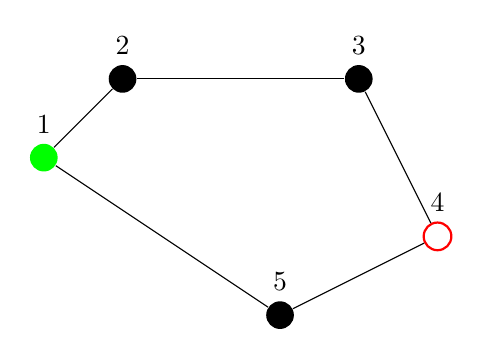
\begin{tikzpicture}
  \tikzset{dot/.style 2 args={circle,fill=#1,inner sep=0,minimum size=10pt,label={above:#2}}}
  \node[dot={green}{1}] (1) at (0,0) {};
  \node[dot={black}{2}] (2) at (1,1) {};
  \node[dot={black}{3}] (3) at (4,1) {};
  \node[dot={none}{4},draw=red,thick] (4) at (5,-1) {};
  \node[dot={black}{5}] (5) at (3,-2) {};

  \draw[thin,black] (1) -- (2);
  \draw[thin,black] (2) -- (3);
  \draw[thin,black] (3) -- (4);
  \draw[thin,black] (4) -- (5);
  \draw[thin,black] (5) -- (1);
\end{tikzpicture}

    \caption{Exemplo de polígono convexo com os vértices indexados em sentido horário. O vértice vermelho sem preenchimento é o mais distante do vértice verde.} \label{SMAWK:Polygon}
\end{figure}

Vamos construir uma matriz~$A$ Monge com~$n$ linhas e~$2n - 1$ colunas tal que, para cada~$i \in [n]$, se~$j$ é uma coluna que atinge o máximo na linha~$i$, então o vértice~$p_{j}$ maximiza~$d(p_i,p_j)$. Para todo índice~$i \in [n]$ de linha de~$A$ e~$j \in [2n - 1]$ de coluna de~$A$ vale que

\begin{equation*}
A[i][j] = \begin{cases}
d(p_i,p_j) & \text{, se } i < j < i+n \text{,} \\
-C|j - i| & \text{, se } j \leq i \text{ e } \\
-C|j - n - i| & \text{, se } i + n \leq j \\
\end{cases}
\end{equation*}
onde~$C$ é uma constante maior do que qualquer distância entre um par de vértices do polígono. É suficiente tomar~$C = \max\limits_{i \in [n]}\{d(p_i,-p_i)\}$, por exemplo, o que pode ser calculado em tempo~$\Cl{O}(n)$.

Primeiro, já que em cada linha~$i$ existe uma entrada~$d(p_i,p_j)$ para cada~$j \in [n]$ onde~$i \neq j$ e estas são as únicas entradas positivas da linha, é verdade que, se uma coluna~$j$ alcança um máximo nesta linha, ele maximiza a distância~$d(p_i,p_j)$. Se provarmos que a matriz~$A$ descrita é totalmente monótona por linhas, mostramos que o Problema~\ref{SMAWK:TPMD} pode ser resolvido em tempo~$\Cl{O}(n)$ com o algoritmo~\textsc{SMAWK}.

\begin{figure}[h]
    \centering
    \begin{tikzpicture}

\definecolor{c}{rgb}{1,0.3,0.3}
\matrix[matrix of nodes, column sep=5pt, row sep=1pt] (m) {
  \textcolor{c}{0} & 2 & 17 & 26 & 13 & \textcolor{c}{0} & \textcolor{c}{-104} & \textcolor{c}{-208} & \textcolor{c}{-312} \\
  \textcolor{c}{-104} & \textcolor{c}{0} & 9 & 20 & 13 & 2 & \textcolor{c}{0} & \textcolor{c}{-104} & \textcolor{c}{-208} \\
  \textcolor{c}{-208} & \textcolor{c}{-104} & \textcolor{c}{0} & 5 & 10 & 17 & 9 & \textcolor{c}{0} & \textcolor{c}{-104} \\
  \textcolor{c}{-312} & \textcolor{c}{-208} & \textcolor{c}{-104} & \textcolor{c}{0} & 5 & 26 & 20 & 5 & \textcolor{c}{0} \\
  \textcolor{c}{-416} & \textcolor{c}{-312} & \textcolor{c}{-208} & \textcolor{c}{-104} & \textcolor{c}{0} & 13 & 13 & 10 & 5 \\
};
\end{tikzpicture}

    \caption{Matriz~$A$ referente ao polígono da Figura~\ref{SMAWK:Polygon} com o quadrado da distância euclideana. Os valores em vermelho são os da forma~$-C|x|$ para algum inteiro~$x$.}
\end{figure}

\begin{prop}
A matriz~$A$ descrita é totalmente monótona côncava por linhas.
\end{prop}

\begin{proof}
Assuma que~$n > 2$. Os dois casos restantes são triviais. Vamos mostrar que para qualquer escolha de índices~${ i \in [n-1] }$ e~${ j \in [2n-2] }$ vale a desigualdade~${ A[i][j] + A[i+1][j+1] \geq A[i][j+1] + A[i+1][j] }$. Se~$i > j$, então a desigualdade equivale a~${ -C(i - j) - C(i + 1 - j - 1) \geq -C(i - j - 1) - C(i + 1 - j) }$. O caso onde~${ j > i + n} $ se desenvolve de maneira similar.

Considere agora o caso onde~$i = j$ ou~$i = j + n$. Vale que~$A[i][j] = A[i+1][j+1] = 0$, portanto, o lado esquerdo da desigualdade soma 0. Devemos provar que~$0 \geq A[i+1][j] + A[i][j-1]$. Nas duas situações, o lado direito desta desigualdade é a soma da distância entre dois vértices do polígono e~$-C$. Pela escolha de~$C$, a desigualdade vale. Nos casos onde~$i + 1 = j$ ou~$i + n - 1 = j$, é possível escolher vértices~$a,b$ e~$c$ do polígono de forma que a desigualdade proposta seja equivalente a~$d(a,b) + d(b,c) \geq d(a,c)$, que é a desigualdade triangular. Se~$i+1 = j$, escolhemos~$a = p_i$,~$b = p_{i+1}$ e~$c = p_{i+2}$. Se~$i+n-1 = j$, escolhemos~$a = p_{i+1}$,~$b = p_{i+n-1}$ e~$c = p_{i}$.

Resta provar o caso onde~$i + 1 < j < i + n - 1$. Neste caso os vértices~$p_i,p_{i+1},p_j$ e $p_{j+1}$ são todos distintos e estão listados, nesta sequência, em sentido horário. Isso faz com que os segmentos~$p_ip_j$ e~$p_{i+1}p_{j+1}$ se intersectem. Tome o ponto~$t$ de intersecção. É fácil perceber que o lado esquerdo da desigualdade equivale a~$d(p_i,t) + d(t,p_j) + d(p_{i+1},t) + d(t,p_{j+1})$. Pela desigualdade triangular, isto é maior ou igual a~$d(p_i,p_{j+1}) + d(p_{i+1},p_j)$, o lado direito da desigualdade.

Pelo Teorema~\ref{Monge:theo+1}, provamos que~$A$ é Monge côncava. Pelo Teorema~\ref{Monge:MCtoTM}, provamos que~$A$ é totalmente monótona nas linhas.
\end{proof}

É interessante observar que, na construção realizada acima, a matriz~$A$ é Monge côncava e possui valores potencialmente grandes em módulo, já que precisamos realizar a escolha do valor~$C$ de forma que ele supere todos os outros valores da matriz. Aggarwal, Klawe, Moran, Shor e Wilber~\cite{Aggarwal:1987} mostram uma forma de construir uma matriz parecida com a~$A$ que é apenas totalmente monótona (não Monge) e também pode ser utilizada para resolver o problema proposto na mesma complexidade. A ausência de valores desnecessariamente grandes como os que ocorrem na matriz modelada aqui pode ajudar a evitar complicações numéricas na aplicação do algoritmo.

Além de aplicações em geometria, o algoritmo SMAWK, bem como a otimização da divisão e conquista, é útil na agilização de problemas de programação dinâmica~\cite{Galil:1989,Galil:1992}. No Capítulo~\ref{Monge} foi apresentado o Problema~\ref{ Monge:example }, formulado com programação dinâmica e resolvido com o algoritmo~$\SMAWK$, por exemplo.
